% English manuscript. Source of truth for the text: docs/paper_draft_en.md (converted 2026-10-20).
% Compile with XeLaTeX (Overleaf: Menu > Compiler > XeLaTeX; latexmkrc in this folder also selects it).
% Numbers come from results/*.csv; figures from scripts/2026-10-20/make_figures.py.
\documentclass[11pt]{article}
\usepackage[a4paper,margin=2.5cm]{geometry}
\usepackage{fontspec}
\usepackage{amsmath,amssymb}
\usepackage{graphicx}
\usepackage{booktabs,tabularx,array,multirow}
\usepackage[numbers,sort&compress]{natbib}
\usepackage{enumitem}
\usepackage{caption}
\usepackage[section]{placeins}
\usepackage{xcolor}
\usepackage{xurl}
\usepackage[hidelinks]{hyperref}
\captionsetup{font=small,labelfont=bf}
\graphicspath{{figures/}}
\newcolumntype{L}{>{\raggedright\arraybackslash}X}
\newcommand{\code}[1]{\texttt{#1}}
\setlist{itemsep=2pt,topsep=4pt}
\setlength{\emergencystretch}{3em}

\title{Failure Prediction in Small Qwen Language-Model Agents:\\Hidden-State Probes Do Not Beat Visible Information}
\author{Author information withheld for review}
\date{Draft, \today}

\begin{document}
\maketitle

\begin{abstract}
Linear probes on the hidden states of language-model agents have been proposed as cheap monitors that predict failure early, but their gains have been measured against baselines that do not see the task.
We tested whether such probes predict failure beyond the information visible in the prompt for a 3-billion-parameter Qwen2.5 agent in the ALFWorld household text environment.
We evaluated between games on 500 greedy episodes and within games on 100 games run eight times each, compared the probe with a ladder of baselines built from the task type, the prompt text and progress features,
split all data by room layout, and fixed the primary analysis before running it once.
In the pre-registered comparison the probe was below the full baseline at the first three actions by 0.13 to 0.18 in area under the receiver operating characteristic curve (all 95\% confidence intervals below zero),
and on 250 held-out games no action was superior (differences from $-0.029$ to $+0.039$, all intervals including zero).
The game explained 69.5\% of the outcome variance (95\% confidence interval 61.3--76.5\%). Within games, the probe and the baselines all separated failed from successful attempts above chance from the third action,
but the probe was superior in none of six comparisons. A four-billion-parameter Qwen3 agent and an external prompt gave the same result, with no superior action in either.
Used to stop failing episodes, the probe was not shown to save more actions than a fixed limit (difference $-0.032$, 95\% confidence interval $-0.183$ to $+0.119$).
In this setting, hidden states did not add to visible information; claims of hidden-state failure signals in agents should be tested against baselines that see the task and within tasks.
\end{abstract}

\section{Introduction}
Language-model agents interact with an environment over many steps, and an episode that ends in failure consumes as much computation as one that succeeds. The cost matters most where agents run locally.
On consumer devices, agentic execution raises power draw, temperature and battery drain well above single-inference use, and a substantial amount of this energy is spent on runs that do not succeed~\cite{pham2026agentstop}.
In our setting, a Qwen2.5-3B agent solved 22.4\% of the first 250 ALFWorld games (56/250; Wilson 95\% CI 17.7--28.0\%), and failed episodes accounted for 89.7\% of the executed steps in these games.
Stopping doomed episodes early could recover much of this cost. For a small agent, however, the monitor itself has to be cheap. A 0.6B text monitor adds only 0.1--0.6\% compute to the three open-weight 9--31B policies in Fail-Fast~\cite{wang2026failfast}.
Under the same parameter-proportional approximation, a 0.5B monitor would add about 13--16\% to a 3B actor, and a 7B monitor would cost about 2.4 times as much as the actor.
A probe on the hidden states that the actor already computes needs no additional model call, which makes it a natural candidate for small agents, provided that it really predicts failure.

Predicting failure from internal representations began at the level of questions. Language models can predict whether they know the answer to a question~\cite{kadavath2022know}. The entropy over the meanings of sampled answers predicts accuracy~\cite{kuhn2023semantic},
and linear probes approximate that entropy from the hidden state of a single generation~\cite{kossen2024sep} or from the question alone, before any token is generated~\cite{moreno2026noanswer}. Ruan et al.~\cite{ruan2026doomed} extended probing to multi-step agents.
They trained a linear probe on the hidden state at the last token of an action and reported that it predicts eventual failure from the first rounds (round-1 AUC 0.86 and 0.81 on TextCraft with two of three models)
and is consistently stronger than a scorer built from behavioral features. In parallel, early-termination systems based on token log-probabilities~\cite{pham2026agentstop}, a small text monitor~\cite{wang2026failfast}, and behavioral and textual features~\cite{shi2026earlyeval} have been proposed.

These reports leave one question open: does the signal show how the current attempt is going, or does it show which task the agent faces? Four limitations prevent an answer.

First, outcomes are largely determined by the task. In ten repeated runs of Llama-3.1-70B on HotpotQA, 64 of 100 questions were answered correctly in every run and 23 in none, and linear probes could not predict per-run correctness (AUC 0.34--0.56)~\cite{mehta2026commit}.
In our data, the game explains 69.5\% of the outcome variance (95\% CI 61.3--76.5\%; the games were stratified by greedy outcome, so this is not a population value). A pooled AUROC can then reflect which task it is rather than how the attempt is going.
Bulut~\cite{bulut2026problem} showed that the pooled AUROC is a weighted sum of a within-task and a between-task component, and that a predictor depending on the task alone scores exactly 0.5 within a task.
Reconstructing the closest published early-window probe on public MATH generations, he obtained a pooled AUROC of 0.849 but only 0.496 (95\% CI 0.466--0.527) within problem, and a pre-registered difficulty-controlled test found no gain.
Activations taken before generation have also been reported to encode a model-specific notion of difficulty~\cite{lugoloobi2026failures}. Ruan et al.\ collected 4--8 rollouts per task but report no within-task evaluation or difficulty control.

Second, the comparison baselines are weak. The behavioral scorer in~\cite{ruan2026doomed} uses only action log-probabilities, token counts, prefix length and error keywords; it has no access to the task statement, the observations or the progress made.
In our data, the task type alone gives an AUROC of 0.603 before the first action. In another study, the similarity of observed text predicted behavioral variability better than the similarity of hidden states ($r=-0.63$ versus $-0.35$)~\cite{mehta2026commit}.

Third, the within-task control of~\cite{bulut2026problem} does not carry over to interactive agents. Rollouts of the same game in a discrete-action environment share identical prompts early on, which produces tied pairs (52--70\% of our evaluation pairs)
and caps the attainable AUROC. In our data, bootstrap intervals also proved narrower than their nominal level (80--94\% coverage against 95\%). The analysis in~\cite{bulut2026problem} covers single-generation math reasoning and does not address these issues.

Fourth, the cost argument for monitors assumes a large policy. The 0.1--0.6\% overhead in~\cite{wang2026failfast} holds for 9--31B policies, and the assumption fails for the 3B-class agents that run on consumer devices.

\textbf{The core problem is therefore that existing evidence cannot tell whether hidden-state failure signals in agents read in-progress failure or task difficulty and visible information. As a result, it is unknown whether the cheapest monitor available to a small agent is useful.}

The distinction decides what to deploy. If a probe reads only difficulty, a classifier on the task text is enough and no access to model internals is needed. If it reads in-progress failure within a task, it offers a gain that visible information cannot provide.
The same distinction also determines whether the probe supports early stopping.

We therefore evaluate hidden-state failure prediction in a small ALFWorld agent~\cite{shridhar2021alfworld} under controls that address each limitation. Each limitation is matched with a required function and a design component:
\begin{enumerate}
\item \emph{Separate difficulty from in-progress failure.} We evaluate at two levels: a task level (greedy decoding, 500 games) and an attempt level (100 games $\times$ 8 rollouts at temperature 1, scored by within-game pairwise AUROC), together with a difficulty oracle that scores exactly 0.5 within a game.
\item \emph{Measure the gain over visible information.} We compare against a five-rung baseline ladder (step index; + task type; + repetition and chosen-action probability; + progress; + TF-IDF of the prompt), plus time-matched variants that drop information from the current step.
\item \emph{Prevent leakage between games.} Games in ALFWorld share room layouts, so we cross-fit and bootstrap by scene. Splitting by game inflated AUROC to 0.97 for a synthetic feature that contained only scene information.
\item \emph{Make the within-task statistics valid for agents.} We report the share of tied pairs and the AUROC ceiling it implies, add a secondary analysis restricted to non-tied pairs, and check the coverage of the intervals with permuted labels.
\item \emph{Prevent selection after seeing results.} The primary analysis and decision rules were registered and run once, and a setting chosen after exploration was confirmed on 250 new games.
\item \emph{Fit a small-agent setting.} The probe reads the 3B actor's own hidden state at no additional model call, actions are chosen by candidate scoring, and we vary the actor (Qwen3-4B), the prompt (the original ReAct examples~\cite{yao2023react}) and, in an exploratory analysis, the size of the reader that reads the actor's trajectory (0.5B--7B).
\end{enumerate}

We did not reuse existing methods unchanged, for three reasons. The protocol of~\cite{ruan2026doomed} controls neither difficulty nor visible information and splits by task, which leaks scene information in ALFWorld.
The within-problem evaluation of~\cite{bulut2026problem} assumes independent single generations, so it cannot handle shared prefixes in sequential environments. The text monitors of~\cite{wang2026failfast} and~\cite{pham2026agentstop} assume a policy large enough that the monitor's cost is negligible.
Small models also often produce actions that are not in the admissible list when they generate freely, so we choose actions by the log-probability of each admissible candidate and reuse the prompt's key--value cache, which lets the agent run on a single 12\,GB GPU.

Under these controls, the probe did not outperform the visible-information baseline. In the pre-registered task-level comparison, the probe scored below the five-rung baseline (differences $-0.181$, $-0.133$ and $-0.159$ at steps 0--2; all 95\% CIs below zero).
In a confirmatory hold-out, no step was superior ($+0.039$, $+0.035$, $-0.029$; all CIs include zero). Within a game, both the probe and the baselines predicted failure better than chance from step 2 (probe AUROC 0.585 and 0.619 at steps 2 and 3),
but the probe was superior in none of six comparisons. The same pattern appeared with another actor (Qwen3-4B, superior in 0/3 comparisons) and another prompt (ReAct, 0/3; inferior at step 2).
Used to stop doomed episodes, the probe was not shown to save more steps than a fixed step cap at up to 10\% lost successes (difference $-0.032$, 95\% CI $-0.183$ to $+0.119$).
These results do not show that the probe and the baseline are equivalent: the intervals are wide (about $\pm$0.06--0.10 at the task level), and we tested one environment and two prompts.

Our contributions are as follows.
\begin{itemize}
\item We re-examine hidden-state failure prediction for multi-step agents under difficulty control and within-task evaluation, and find no evidence that the probe beats visible information in this setting.
\item We provide pre-registered comparisons of a hidden-state probe against a baseline ladder of visible information, using the same splits and statistics throughout.
\item We quantify two problems that arise when within-task evaluation is applied to discrete-action agents: tied pairs from shared prefixes, and bootstrap intervals that are narrower than nominal.
\item We compare readers of different sizes on identical trajectories by separating the actor from the reader. This part is exploratory, and no monotone trend with size was observed.
\end{itemize}

\section{Related Work}
We group prior work by what the predictor reads and what it is compared against. We then state which parts of earlier protocols we reuse.

\subsection{Predicting correctness from internal representations}
Work on reading success or failure from a model's own states began at the level of single questions. Kadavath et al.~\cite{kadavath2022know} trained a value head to predict P(IK), the probability that the model knows the answer to a question, without reference to any proposed answer.
P(IK) transferred partially across tasks but was poorly calibrated out of distribution. Kuhn et al.~\cite{kuhn2023semantic} measured uncertainty as the entropy over meaning clusters of several sampled answers, which predicted accuracy better than lexical baselines, but it required multiple generations per question.
Kossen et al.~\cite{kossen2024sep} removed that cost by training linear probes on the hidden state of a single generation to approximate the semantic entropy; the probes generalized better out of distribution than probes that predict accuracy directly.
Moreno Cencerrado et al.~\cite{moreno2026noanswer} moved the readout before generation: probes on activations taken after the question is read, in models from 7B to 70B parameters, predicted whether the forthcoming answer would be correct, but generalization faltered on mathematical reasoning questions.
Lugoloobi et al.~\cite{lugoloobi2026failures} trained linear probes on pre-generation activations to predict policy-specific success on math and coding tasks; the linear probe scored above TF-IDF and above question length in 14 of the 15 settings of their main results table, and the authors concluded that models encode a model-specific notion of difficulty distinct from human difficulty. In all of these studies the target is defined per question, either as one outcome or as an aggregate over samples.
Such a target is meaningful for question answering, but it does not separate a hard question from a failing attempt.

\subsection{Hidden-state monitors for agents}
Ruan et al.~\cite{ruan2026doomed} applied probing to multi-step agents. They placed a linear probe on the residual stream at the last token of each action, with one layer fixed per model--environment cell.
Probes were cross-fitted with task-grouped splits and evaluated per round on TextCraft and WebShop (800 episodes per cell, three agents of 1.7B--7B parameters).
They reported that the probe predicts eventual failure from the first rounds and outperforms a scorer built from behavioral features. They then converted the signal into an abort cascade with a recall guarantee.
ALFWorld appears in their work only as a boundary test with Qwen-2.5-7B (477 rollouts; probe AUC 0.815) and Qwen3-1.7B (0.764). Their probe, replay procedure and task-grouped evaluation are close to ours.
Their behavioral scorer, however, uses only action log-probabilities, token counts, prefix length and error keywords. Their study reports no within-task evaluation or difficulty control, even though it collected 4--8 rollouts per task, and the grouped splits remain in-distribution by their own account.

Other agent studies read hidden states for different targets. Khan and Khan~\cite{khan2026companion} built a probe-based monitor on layer-28 hidden states of Gemma 4 E4B that detects reasoning degradation at no measured inference overhead.
The probe was trained on 35 proxy-labeled examples drawn from the task bank later used for evaluation, and the authors present the work as a feasibility study. Their small-model tests (1B--1.5B) showed no improvement.
Mehta and Datta~\cite{mehta2026commit} measured the similarity of hidden states across repeated runs at the same step and related it to behavioral stability in ReAct agents ($r=-0.35$ at step 4 on Llama-3.1-70B).
They reported that shared retrieved evidence explains much of the association, that observation text predicts behavior better, and that the measure indexes stability rather than correctness. Linear probes in the same study could not predict per-run correctness.

\subsection{Early termination without internal states}
A second line of work stops likely failures from observable signals. AgentStop~\cite{pham2026agentstop} trains gradient-boosted trees on token log-probability features and measures energy on a consumer laptop.
It reduced wasted energy by 15--20\% for Qwen3-30B-A3B with less than a 5\% utility drop. In the 1.7B model, however, log-probabilities of failed and successful runs overlapped more.
Fail-Fast~\cite{wang2026failfast} fine-tunes a 0.6B model on text prefixes of SWE-bench Verified trajectories. At a 5\% false-positive budget it saved 20.4\% of tokens for Qwen3.6-27B, against 12.5\% for an AgentStop adaptation and 11.4\% for a control that uses the step count alone.
During training it pairs successful and failed prefixes matched by progress to control for instance difficulty. Its evaluation, however, pools 100 held-out instances $\times$ 5 runs, and we found no within-instance analysis.
EarlyEval~\cite{shi2026earlyeval} applies the same idea to evaluation cost, halting benchmark runs with classifiers over behavioral, textual and reference-solution features (13--26\% fewer steps).
Pan et al.~\cite{pan2026monitoring} showed that observable macro and micro trajectory features are competitive with internal-signal baselines for web agents, with task-grouped cross-validation.
These monitors read observable signals (log-probabilities, text and behavior), and all of their evaluations are pooled over tasks. Their monitors are cheap only relative to large policies: the 0.1--0.6\% overhead in~\cite{wang2026failfast} holds for three open-weight 9--31B policies.

\subsection{Task difficulty as a confound}
The strongest argument that pooled scores can mislead comes from Bulut~\cite{bulut2026problem}. He showed that a pooled AUROC is a weighted sum of a within-problem and a between-problem component, and that any predictor that depends on the problem alone scores exactly 0.5 within a problem.
A trace-blind difficulty proxy reached AUROC 0.873 on 192K public R1 generations. A reconstruction of the closest published early-window probe scored 0.849 pooled but 0.496 (95\% CI 0.466--0.527) within problem, and a pre-registered test found no gain over a difficulty baseline.
Mehta and Datta~\cite{mehta2026commit} reached a similar conclusion for agents from the other direction: correctness was largely determined by the question (64 of 100 questions always correct, 23 never), and per-run probes failed.
Both studies concern settings in which the same question is answered independently, either as a single generation~\cite{bulut2026problem} or as a few ReAct runs~\cite{mehta2026commit}. Neither evaluates a hidden-state failure probe for an agent that acts in an environment.

\subsection{Positioning}
We reuse from~\cite{ruan2026doomed} the teacher-forced replay, the per-round evaluation, and the grouping of splits. From~\cite{bulut2026problem} we take the within-problem pairwise AUROC and the use of a baseline that depends on the task alone. From~\cite{wang2026failfast} we take the control that uses the step count alone.
We add what these works lack for small interactive agents: a five-rung baseline ladder that gradually adds visible information, evaluation at two levels (across games and within a game), scene-level grouping,
handling of tied pairs and of interval coverage in discrete-action environments, and a comparison of a probe on the actor's own hidden state against monitors whose cost is counted relative to a 3B actor.

\section{Method}

\subsection{Environment and agent}
We used ALFWorld (TextWorld version, \code{alfworld} 0.4.2) with the 3,553 games of the training split and all six task types.
An episode ended when the task was completed or after 30 actions; episodes that did not complete the task were labeled as failures (label 1).
Because ALFWorld has no failing terminal state, a failure is a timeout. To check the 30-action limit, we re-ran all 399 greedy failures with a limit of 100 actions under a pre-registered rule:
11 of 399 succeeded between actions 31 and 100 (2.8\%, Wilson 95\% CI 1.6--4.9\%), so the upper bound was below the pre-registered 5\% threshold and we kept the 30-action label (sensitivity analyses in Section~\ref{sec:robust}).
The agent (actor) was Qwen2.5-3B-Instruct in bfloat16. At each step the prompt contained a fixed system message (rules and one worked example episode),
the task sentence, the last six observation--action pairs, the current observation, the actions that had recently produced no effect, and the list of admissible actions.
We call this prompt v2. It was written by us: an earlier version followed the thought--action format of ReAct~\cite{yao2023react}, and when we switched to candidate scoring we dropped the thought step
and added six rules and one handwritten example episode. None of its text is taken from the ReAct exemplars. A second, external prompt is described in Section~\ref{sec:actors}.

The actor selected actions by constrained scoring rather than free generation. Each admissible action $a$ (excluding \code{help}, \code{inventory} and \code{look})
was scored by the summed log-probability of the continuation \code{Action: a<|im\_end|>} given the prompt, computed in one batched pass that reuses the prompt's key--value cache.
In the greedy policy the highest-scoring action was taken. In the sampling policy an action was drawn from $\mathrm{softmax}(\text{score}/T)$ with $T=1$,
i.e.\ the model's distribution renormalized over admissible actions; the random generator was seeded by (sample seed, episode index, step), so rollouts are reproducible and resumable.
Free generation was not used because small models frequently produced inadmissible actions in preliminary runs (Appendix Table~\ref{tab:a5}).

\subsection{Representations: separating the actor from the reader}
Hidden states were taken at the last prompt token, immediately before the action is scored, at relative depths of 25, 50, 75 and 100\% of the layers
(layers 9, 18, 27 and 36 for the 3B model). To vary model size without changing the trajectories, we passed the actor's stored prompts through \emph{reader} models by teacher forcing:
Qwen2.5-0.5B-, 1.5B- and 3B-Instruct in bfloat16, and Qwen2.5-7B-Instruct with 4-bit NF4 weights (bfloat16 compute), the largest that fits in 12\,GB of GPU memory.
All four models share the tokenizer and chat template; the re-tokenized prompt length matched the stored length at every step, and on the steps we checked (five) the 3B reader reproduced the actor's stored hidden states exactly.
Because readers other than 3B read another model's trajectories, results for them concern external monitoring, not self-monitoring.

\subsection{Data}
\paragraph{Task-level data (greedy).} We collected 500 greedy episodes on distinct games in the environment's deterministic order.
The first 250 episodes were used for the pre-registered and exploratory analyses; episodes 250--499 were collected afterwards as a confirmatory hold-out
for a single comparison fixed before collection (Section~\ref{sec:stats}). Reader hidden states were extracted for the first 250 episodes.

\paragraph{Attempt-level data (sampling).} Under greedy decoding the outcome is a function of the game, so task-level labels cannot separate task difficulty from in-progress failure.
We therefore re-ran 100 games eight times each with the sampling policy: a pilot of 20 games (10 games the greedy policy solved, 10 it failed; sample seed 0)
and a main set of 80 new games (40 solved, 40 failed by the greedy policy, drawn at random with seed 1 from the remaining greedy games; sample seed 1).
Stratifying by the greedy outcome was decided after the pilot and is reported as a selection step. In total 800 rollouts were used.
Re-collecting the first 24 main-set rollouts on a fresh installation reproduced them exactly (actions, outcomes and hidden states).

\subsection{Evaluation units}
\paragraph{Task level (between games).} For each round $r$ we kept one row per episode still running at step $r$ and computed the AUROC for predicting failure.
Within a round the step index is constant, which removes episode length as a predictor. The pre-registered rounds 1--3 are steps 0--2 (the first three actions);
every episode was still running at these steps.

\paragraph{Attempt level (within games).} All rollouts of a game share the step-0 prompt, so step 0 was excluded and steps 1--3 were evaluated.
Only games with at least one success and one failure among their eight rollouts contribute. The metric is the within-game pairwise AUROC:
over all (failed, successful) rollout pairs from the same game, the fraction in which the failed rollout received the higher failure score (ties count one half),
pooled across games with weights proportional to the number of pairs.

Two properties of this design were checked before the attempt-level results were read. First, sampled rollouts of a game often had not diverged yet:
of the 470 evaluation pairs per step (39 games with both outcomes, 28 scenes), 70.4\%, 66.4\% and 52.3\% had identical prompts at steps 1, 2 and 3.
The probe input is then identical, so these pairs are ties and cap the probe's pairwise AUROC at 0.648, 0.668 and 0.739.
Second, rungs 3--5 include the repetition count and the probability of the action sampled at the current step, which lie after the probe's input in time
and are exactly where rollouts diverge. We therefore pre-specified two secondary analyses: (i) the same metric restricted to pairs whose prompts differ,
and (ii) time-aligned rungs 4t and 5t in which those two features are taken from the previous step. Secondary results are reported after, and do not replace, the primary result.

\subsection{Predictors}
\paragraph{Probe.} Standardization followed by L2-regularized logistic regression with balanced class weights.
The regularization strength $C \in \{10^{-4}, 10^{-3}, 10^{-2}, 10^{-1}, 1\}$ was selected in a nested three-fold cross-validation inside each training fold.
A one-hidden-layer MLP (64 units, $\alpha = 10^{-2}$, early stopping, fixed hyperparameters) was evaluated as an exploratory probe.

\paragraph{Baseline ladder.} Each rung adds information available without hidden states:
(1) step index; (2) + task type; (3) + recent repetition count, probability of the chosen action and number of candidates;
(4) + progress features computed from earlier actions (distinct locations visited, open/take/transform/move counts, whether the target object has been seen);
(5) + TF-IDF (word 1--2-grams) of the full user message, which contains the task sentence, room description, recent history, current observation and admissible actions.
Rung 3 uses quantities computed after scoring the current step, slightly later than the probe's input; this favors the baseline.
The probe is compared with rung 5 (pre-registered) and, at the attempt level, with rungs 4 and 5.

\paragraph{Difficulty oracle (attempt-level analysis).} Each game's greedy outcome from the task-level data, which is independent of the sampled rollouts.
It is constant within a game, so its within-game AUROC is 0.5 by construction (verified as an implementation check).
We also report the share of outcome variance explained by the game ($\eta^2$) and, on rows pooled across games, the AUROC gain of a logistic stack of [oracle, predictor] over the oracle alone.

\subsection{Cross-fitting, statistics and pre-registration}\label{sec:stats}
All predictors were cross-fitted with five-fold stratified group splits by \textbf{scene} (the ALFWorld floor plan; 86 scenes in the first 250 games),
repeated with two seeds and averaged, so that every row is scored by a model that never saw its scene. Splitting by game instead inflated AUROC to 0.97
on a synthetic feature that encodes only the scene. Standardization, TF-IDF and model selection were fit inside each training fold.

Task-level 95\% confidence intervals use a scene-level cluster bootstrap (1,000 resamples); differences between a probe and a baseline are computed on the same resamples.
The null distribution re-runs the full pipeline, including nested selection, on permuted labels (100 permutations).
Attempt-level intervals use a game-level bootstrap (1,000 resamples), and the null permutes labels within games with scores held fixed (1,000 permutations).

Before any probe was fit we fixed the code commit, configuration and primary analysis (3B actor and reader, 50\% depth, linear probe, rounds 1--3, comparison with rung 5),
and ran it once. Every later analysis on the same episodes is labeled exploratory. A single exploratory configuration (75\% depth, linear) was then tested on the confirmatory
hold-out, training on all 500 episodes and evaluating only episodes 250--499. The decision rule was: superior if the lower 95\% bound of the difference exceeds 0,
non-inferior if it exceeds $-0.05$, inferior if the upper bound is below 0, otherwise inconclusive. The margin of 0.05 was chosen after the exploratory analysis.
The attempt-level analysis (75\% depth, linear, vs.\ rungs 4 and 5, steps 1--3) and its interpretation table were fixed before the sampled rollouts were collected.
All changes to the frozen procedures are logged with dates in the repository.
Interim counts of the 100-action re-run were seen twice before its decision (at most 3 late successes among the first 116 games); the decision rule had been committed beforehand and was not changed.

\subsection{Compute}
One NVIDIA RTX 4070 (12\,GB) under WSL2 (Ubuntu 22.04), Python 3.11, PyTorch 2.11 (CUDA 12.8), Transformers 5.19.0.
Collecting one episode took about 8--11\,s; the 640 main-set rollouts took 88\,min.

\paragraph{Monitor cost.} Following~\cite{wang2026failfast}, we approximate inference compute as $2N$ floating-point operations per token for a model with $N$ parameters, so the extra cost of a separate monitor that reads the same tokens is its parameter count relative to the actor's.
With the public Qwen2.5 counts (0.5B: 0.49B total, 0.36B without embeddings; 3B: 3.09B and 2.77B; 7B: 7.61B and 6.53B), a 0.5B monitor adds $0.36/2.77 \approx 13\%$ to $0.49/3.09 \approx 16\%$ to a 3B actor,
and a 7B monitor costs $6.53/2.77 \approx 2.36$ to $7.61/3.09 \approx 2.46$ times as much as the actor (about 2.4 times). A probe on the actor's own hidden state adds one dot product with a 2,048-dimensional vector per step and needs no additional model call.
We did not measure energy or latency.

\section{Results}
\subsection{Task level}\label{sec:task}
\paragraph{Data.} The greedy actor completed 56 of the first 250 episodes (22.4\%, Wilson 95\% CI 17.7--28.0\%) and 101 of all 500.
The 250 games covered 86 scenes. Successful episodes took 4--28 actions (median 12), so all 250 episodes were still running at steps 0--3,
and the failure rate in every pre-registered round was 0.776.

\paragraph{Baselines.} Information visible without hidden states already predicted failure before the first action (Table~\ref{tab:ladder}, Fig.~\ref{fig:ladder}).
Task type alone gave an AUROC of 0.603, and the full rung-5 baseline reached 0.701 at step 0, 0.732 at step 1 and 0.823 at step 2.
Progress features (rung 4) accounted for most of the rise from step 2 onward ($0.673 \rightarrow 0.834$); at steps 2 and 3, rung 5 was not higher than rung 4.
The step-index rung was exactly 0.500 in every round, as intended. Permuted-label AUROCs averaged 0.50 (95\% range about 0.38--0.62).

\paragraph{Pre-registered comparison.} In the single pre-registered run (3B reader, 50\% depth, linear probe), the probe scored below the rung-5 baseline in all three rounds,
and every 95\% interval of the difference lay below zero (Table~\ref{tab:ladder}, Fig.~\ref{fig:forest}): $-0.181$ ($-0.276$ to $-0.069$) at step 0, $-0.133$ ($-0.230$ to $-0.031$) at step 1 and
$-0.159$ ($-0.240$ to $-0.073$) at step 2. Hypothesis H1 was therefore not supported in the pre-registered cell; this matches the third outcome of the interpretation table fixed in advance
(``even the 3B reader does not beat rung 5'').

\paragraph{Exploratory analyses (same 250 episodes).} We then evaluated all 96 combinations of four readers, four depths, two probe types and three rounds (linear cells in Fig.~\ref{fig:heat}; all cells in Appendix Table~\ref{tab:a6}).
No combination exceeded the baseline by more than 0.004, and the two positive differences ($+0.004$ and $+0.001$) had intervals spanning zero.
The 75\% depth was the best or near-best depth for every reader; for the 3B reader the linear probe at 75\% depth was within $-0.034$ to $-0.011$ of the baseline (all intervals include zero).
Averaged over steps 0--2, the best-depth linear AUROC was 0.660 (0.5B), 0.717 (1.5B), 0.727 (3B) and 0.717 (7B, 4-bit; best depth 100\%), i.e.\ no monotonic increase with reader size;
the 7B result is confounded with quantization. Averaged over depths, the fixed MLP was not better than the linear probe (differences $-0.035$ to $-0.004$).
Of 36 pairwise reader comparisons, 4 had intervals excluding zero, close to the about 2 expected by chance, and their signs were inconsistent.
These analyses were chosen after seeing the pre-registered result and are not evidence on their own.

\paragraph{Confirmatory hold-out.} The one configuration carried forward (3B reader, 75\% depth, linear) was evaluated on the 250 new episodes
(205 failures, failure rate 0.82; Table~\ref{tab:confirm}). The differences from rung 5 were $+0.039$ ($-0.030$ to $+0.100$), $+0.035$ ($-0.030$ to $+0.096$) and $-0.029$ ($-0.087$ to $+0.029$) at steps 0--2.
No round met the criterion for superiority and none was inferior; steps 0 and 1 met the non-inferiority rule, whose margin was set after exploration, and step 2 was inconclusive.
The rung-5 baseline was lower on the hold-out than on the first 250 episodes (0.607 vs.\ 0.701 at step 0), which indicates sample-to-sample variation of this size.

\begin{table}[t]
\centering\small
\caption{Failure-prediction AUROC on the first 250 episodes (pre-registered rounds: steps 0--2).}\label{tab:ladder}
\begin{tabularx}{\linewidth}{@{}Lcccc@{}}
\toprule
 & Step 0 & Step 1 & Step 2 & Step 3$^{a}$ \\
\midrule
Rung 1: step index & 0.500 & 0.500 & 0.500 & 0.500 \\
Rung 2: + task type & 0.603 & 0.603 & 0.603 & 0.603 \\
Rung 3: + repetition, chosen-action probability & 0.659 & 0.633 & 0.671 & 0.700 \\
Rung 4: + progress & 0.673 & 0.700 & 0.834 & 0.814 \\
Rung 5: + TF-IDF of prompt & 0.701 & 0.732 & 0.823 & 0.818 \\
Probe, 3B reader, 50\% depth (pre-registered) & 0.520 & 0.599 & 0.665 & -- \\
\addlinespace
Probe $-$ rung 5 & $-0.181$ & $-0.133$ & $-0.159$ & -- \\
\quad (95\% CI) & ($-0.276$, $-0.069$) & ($-0.230$, $-0.031$) & ($-0.240$, $-0.073$) & \\
\bottomrule
\end{tabularx}
\par\smallskip\raggedright\footnotesize
$n = 250$ episodes (194 failures) per round; CIs from a scene-level cluster bootstrap (1,000 resamples). $^{a}$Baselines only. Interval half-widths for single AUROCs were about 0.07--0.09. Step 3 is not a pre-registered round; the probe was not evaluated there. Sources: \code{results/probe\_main\_3b\_primary*.csv}, \code{results/baselines\_main\_3b.csv}.
\end{table}

\begin{table}[t]
\centering\small
\caption{Confirmatory hold-out (episodes 250--499; 3B reader, 75\% depth, linear).}\label{tab:confirm}
\begin{tabularx}{\linewidth}{@{}Lccc@{}}
\toprule
 & Step 0 & Step 1 & Step 2 \\
\midrule
Probe AUROC (95\% CI) & 0.645 (0.547, 0.736) & 0.716 (0.619, 0.810) & 0.729 (0.633, 0.815) \\
Rung 5 AUROC & 0.607 & 0.681 & 0.758 \\
Probe $-$ rung 5 (95\% CI) & $+0.039$ ($-0.030$, $+0.100$) & $+0.035$ ($-0.030$, $+0.096$) & $-0.029$ ($-0.087$, $+0.029$) \\
Decision (margin 0.05, set post hoc) & non-inferior & non-inferior & inconclusive \\
\bottomrule
\end{tabularx}
\par\smallskip\raggedright\footnotesize
$n = 250$ episodes (205 failures). Training used all 500 episodes; evaluation used only the new 250.
\end{table}

\begin{figure}[tbp]
\centering
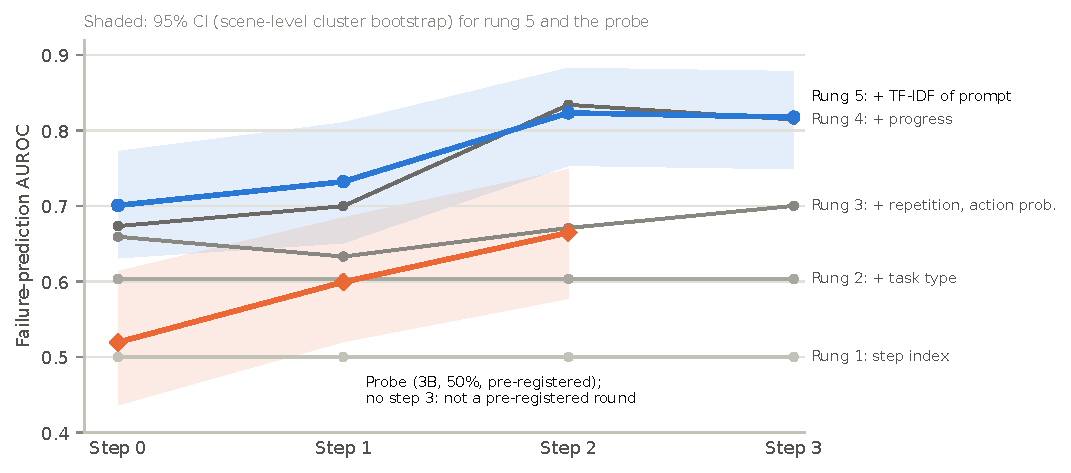
\includegraphics[width=\linewidth]{fig2_baseline_ladder.pdf}
\caption{Failure-prediction AUROC of the baseline ladder (steps 0--3) and the pre-registered probe (steps 0--2) on the first 250 episodes ($n = 250$, 194 failures per step). Rung 5 and the probe are emphasized, with shaded 95\% CIs from a scene-level cluster bootstrap (1,000 resamples); CIs of rungs 1--4 are omitted for legibility. Rung 1 is 0.5 by design and rung 2 does not change with the step. Overlap of the two shaded bands is not a test of their difference; the paired differences are in Fig.~\ref{fig:forest}. Sources: \code{results/baselines\_main\_3b.csv}, \code{results/probe\_main\_3b\_primary.csv}.}\label{fig:ladder}
\end{figure}

\begin{figure}[tbp]
\centering
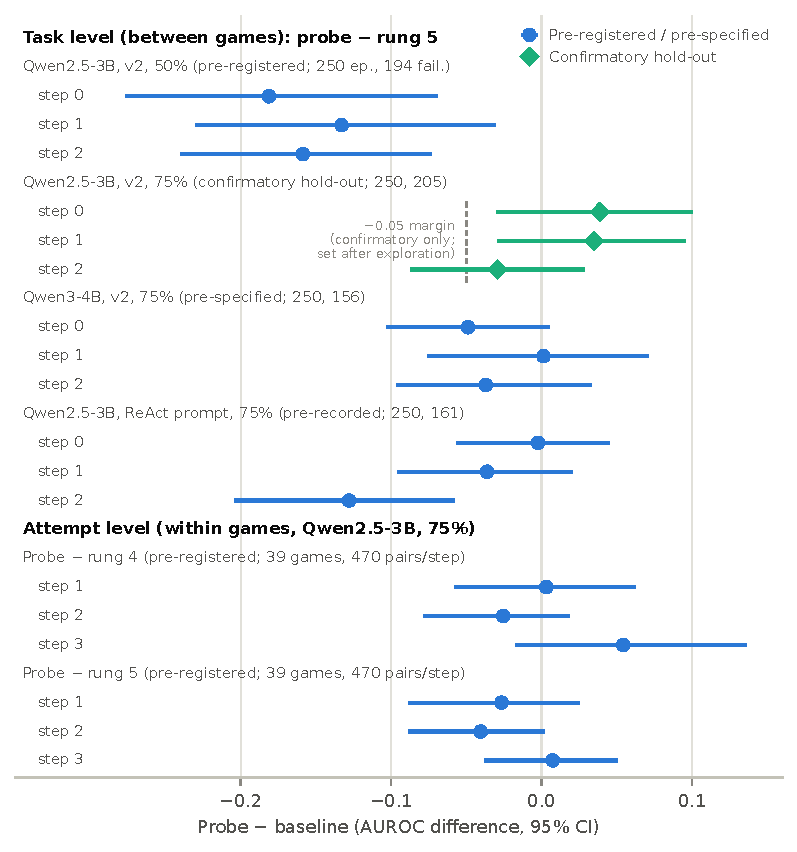
\includegraphics[width=0.82\linewidth]{fig3_probe_minus_baseline.pdf}
\caption{All pre-registered, pre-specified and confirmatory probe-versus-baseline comparisons (18; none superior). Points are AUROC differences with 95\% CIs. Task level: probe $-$ rung 5, scene-level cluster bootstrap (1,000 resamples); labels give the setting and $n$ (episodes, failures). Attempt level: within-game pairwise AUROC differences, game-level bootstrap (1,000 resamples); on label-shuffled data these intervals covered the null value only 80--94\% of the time (Section~\ref{sec:attempt}), so they are too narrow. Dashed segment: $-0.05$ non-inferiority margin, applied only to the confirmatory hold-out and set after the exploratory analysis. Exploratory estimates are not shown (Fig.~\ref{fig:heat}). Sources: \code{results/probe\_main\_3b\_primary\_diff.csv}, \code{confirm\_main\_3b\_diff.csv}, \code{task\_qwen3\_4b\_diff\_p.csv}, \code{task\_react\_qwen25\_3b\_diff\_p.csv}, \code{within\_game\_diff.csv}.}\label{fig:forest}
\end{figure}

\begin{figure}[tbp]
\centering
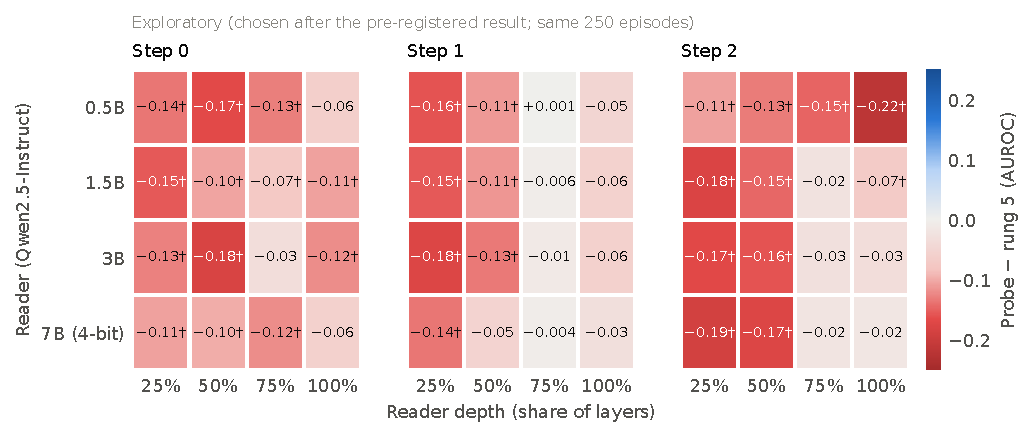
\includegraphics[width=\linewidth]{fig4_reader_depth.pdf}
\caption{Exploratory: probe $-$ rung 5 AUROC difference for every reader $\times$ depth of the linear probe on the first 250 episodes (48 cells, no selection). Diverging color centered on zero (red: probe below rung 5); $\dagger$ marks cells whose 95\% CI (scene-level cluster bootstrap) excludes zero, all of them below zero (31 of 48). No cell's CI lies above zero; the largest difference is $+0.001$. The 7B reader used 4-bit weights, so size is confounded with quantization. MLP cells and CIs: Appendix Table~\ref{tab:a6} and \code{results/explore\_\{0.5B,1.5B,3B,7B-4bit\}\_diff.csv}.}\label{fig:heat}
\end{figure}

\subsection{Attempt level}\label{sec:attempt}
\paragraph{Primary result.} Within games, the probe's pairwise AUROC was 0.520 (95\% CI 0.453--0.583) at step 1, 0.585 (0.522--0.654) at step 2 and 0.619 (0.552--0.687) at step 3 (Table~\ref{tab:within}, Fig.~\ref{fig:forest}).
Rungs 4 and 5 reached 0.517 and 0.547, 0.611 and 0.626, and 0.565 and 0.612. From step 2 on, all three methods separated failed from successful attempts of the same game above chance
(within-game permutation $p \le 0.018$), whereas at step 1 only rung 5 did ($p = 0.016$). None of the six probe--baseline differences met the superiority criterion and none was inferior;
the largest difference was $+0.054$ ($-0.017$ to $+0.136$) against rung 4 at step 3. The result fits no row of the interpretation table cleanly: the probe was not better than the baselines,
and no comparison met the equivalence definition (95\% CI within $\pm 0.05$).

\paragraph{Secondary analyses.} Restricting the evaluation to pairs whose prompts differed (139, 158 and 224 pairs at steps 1--3) raised every method (probe 0.568, 0.753 and 0.750; rung 5 0.633, 0.816 and 0.754),
but none of the six differences was resolved (intervals of about $\pm$0.1--0.2). With the time-aligned rungs 4t and 5t the probe was not better at any step; at step 1 it was lower than both
($-0.045$, $-0.098$ to $-0.006$; $-0.038$, $-0.084$ to $-0.004$), although not after Holm adjustment ($p = 0.18$). Neither tied pairs nor the timing asymmetry therefore explains the absence of a probe advantage.
In all 889 tied pairs the probe and the time-aligned rungs gave identical scores, confirming that they use information from the same point in time.

\paragraph{Calibration of the intervals.} On label-shuffled data (20 seeds), game-level percentile bootstrap intervals contained the null value 80--94\% of the time rather than 95\%,
and the ``equivalent'' verdict appeared in 54--65\% of null runs. Borderline verdicts above should be read with this in mind.

\begin{table}[t]
\centering\small
\caption{Within-game pairwise AUROC ($T = 1$ sampling; 39 games with both outcomes, 470 pairs per step).}\label{tab:within}
\begin{tabularx}{\linewidth}{@{}Lccc@{}}
\toprule
 & Step 1 & Step 2 & Step 3 \\
\midrule
Probe (3B, 75\% depth, linear) & 0.520 (0.453, 0.583) & 0.585 (0.522, 0.654) & 0.619 (0.552, 0.687) \\
Rung 4 & 0.517 (0.452, 0.582) & 0.611 (0.541, 0.687) & 0.565 (0.492, 0.644) \\
Rung 5 & 0.547 (0.478, 0.618) & 0.626 (0.563, 0.699) & 0.612 (0.546, 0.682) \\
Probe $-$ rung 4 (95\% CI) & $+0.003$ ($-0.058$, $+0.063$) & $-0.026$ ($-0.078$, $+0.019$) & $+0.054$ ($-0.017$, $+0.136$) \\
Probe $-$ rung 5 (95\% CI) & $-0.027$ ($-0.088$, $+0.025$) & $-0.040$ ($-0.088$, $+0.002$) & $+0.007$ ($-0.038$, $+0.051$) \\
Tied pairs (identical prompts) & 70.4\% & 66.4\% & 52.3\% \\
\bottomrule
\end{tabularx}
\par\smallskip\raggedright\footnotesize
CIs from a game-level bootstrap (1,000 resamples). Rung 2 and the difficulty oracle are constant within a game and scored exactly 0.500 (implementation check).
\end{table}

\subsection{How much the game determines the outcome}
In the sampled data, the game explained $\eta^2 = 0.695$ (95\% CI 0.613--0.765) of the outcome variance; because games were stratified by their greedy outcome, this is not a population value.
On rows pooled across games, the difficulty oracle alone reached an AUROC of 0.877. Adding the probe to the oracle changed the pooled AUROC by $-0.002$ ($-0.026$ to $+0.025$), $+0.022$ ($-0.005$ to $+0.048$)
and $+0.042$ ($+0.017$ to $+0.073$) at steps 1--3; adding rung 5 changed it by $+0.004$ ($-0.018$ to $+0.027$), $+0.034$ ($+0.007$ to $+0.060$) and $+0.029$ ($+0.003$ to $+0.058$). These gains are uncorrected secondary measures.
Most of what any method predicts across games is therefore already predicted by knowing the game.

\subsection{Other actors and a second prompt}\label{sec:actors}
Each model and prompt is reported separately; results are not pooled.

\paragraph{Which actors entered.} Five further models were piloted on the first 20 games under a rule fixed before the pilots
(at least 3 of 20 successes, completion without running out of 12\,GB of memory, at most three times the reference time per episode, no non-finite hidden states; Appendix Table~\ref{tab:a1}).
Only Qwen3-4B (thinking disabled) passed, with 7 of 20 successes. Qwen3-1.7B, Llama-3.2-3B-Instruct, SmolLM3-3B and Phi-3.5-mini-instruct each succeeded on 1 of 20 games
(Wilson 95\% CI 1--24\%) and were excluded; Phi-3.5-mini also exceeded the time criterion. Before the SmolLM3 pilot we changed the rule so that every model passing it would be included,
so that substitutes could not be chosen after seeing results. Once the pre-listed substitutes were used up we added no further models; the model extension therefore covers two Qwen models.
In the excluded models, actions repeated within the last six steps far more often than in the two Qwen models (66--82\% vs.\ 32--51\%; exploratory description, Appendix Table~\ref{tab:a2}).
Because v2 was tuned with Qwen2.5, this may reflect prompt--model fit rather than model capability; with 20 games per model we make no claim about differences in success rate.

\paragraph{Qwen3-4B, task level.} On the same 250 games the greedy Qwen3-4B actor succeeded on 94 (37.6\%; Qwen2.5-3B: 56).
The depth (75\%) and the comparison with rung 5 were fixed before these data were collected. The probe on the actor's own hidden states did not beat rung 5 in any round
(Table~\ref{tab:settings}): $-0.049$ ($-0.103$ to $+0.005$) at step 0, $+0.001$ ($-0.076$ to $+0.071$) at step 1 and $-0.037$ ($-0.096$ to $+0.033$) at step 2.
No round was superior, also after Holm adjustment across the three rounds, and none was non-inferior or inferior, so all three were inconclusive.
The direction matches Qwen2.5-3B: the probe on the actor's own hidden states shows no advantage over the surface baseline.

\paragraph{Qwen3-4B, attempt level.} Sampled rollouts of Qwen3-4B rarely diverged: only 10 of 50 games had both outcomes among eight rollouts (Qwen2.5-3B: 39 of 100),
and the chosen action had probability above 0.99 in 77\% of steps 1--3. All methods scored 0.47--0.52 within games, with most pairs tied.
We decided before reading these results not to enlarge the sample and to report them only in the appendix (Table~\ref{tab:a3}); the attempt-level question could not be answered for this model.

\paragraph{A second prompt (ReAct exemplars).} To test whether the conclusion depends on our own prompt, we re-ran Qwen2.5-3B on the same 250 games with the original ALFWorld exemplars of ReAct
\cite{yao2023react}, changing only the action grammar to that of \code{alfworld} 0.4.2 (\code{put A in/on B} $\rightarrow$ \code{move A to B}). The two prompts differ in several ways at once (Appendix Table~\ref{tab:a4}):
the ReAct prompt is a raw completion string rather than a chat template, uses two exemplars matched to the current task type instead of one fixed example,
keeps the full history instead of the last six steps, and omits the admissible-action list and the note on failed actions. The policy, games, analysis and decision rule were unchanged,
and the rung-5 text used only the current game, excluding the exemplars. We therefore treat this prompt as a check on the conclusion, not as an estimate of any single prompt factor.

The pre-recorded comparison (75\% depth, linear, vs.\ rung 5; 89 successes) gave $-0.002$ ($-0.057$ to $+0.045$) at step 0, $-0.036$ ($-0.096$ to $+0.021$) at step 1 and $-0.128$ ($-0.204$ to $-0.058$) at step 2 (Table~\ref{tab:settings}).
No round was superior (also after Holm adjustment); steps 0 and 1 were inconclusive and step 2 was inferior. As specified in advance, this shows no evidence that the probe beats the surface baseline
under an external prompt either. We do not compare the size of the gap between prompts, which was not tested and is affected by their different failure rates (0.776 vs.\ 0.644).
At 50\% depth (secondary) the differences were $-0.036$, $-0.032$ and $-0.048$, all inconclusive. Under this setting the ReAct-format prompt succeeded more often than v2
(89 vs.\ 56 of 250; paired difference $+0.132$, 95\% CI 0.060--0.204; exact McNemar $p = 0.0006$); because several factors changed together, we do not attribute this to any one of them.

In an exploratory check, a probe trained on v2 trajectories and applied to ReAct trajectories (scenes of the test games excluded from training) reached 0.527, 0.493 and 0.555 at steps 0--2,
below the probe trained within ReAct (0.659, 0.623 and 0.593; differences at steps 0 and 1 with intervals below zero). Re-standardizing the ReAct states without labels did not help (0.550, 0.482, 0.586).
This suggests that the direction the probe learns is tied to the prompt format; because the two prompts also extract hidden states at different tokens, we cannot separate a different signal from a shifted representation.

\paragraph{Summary across settings.} In the four task-level evaluations (pre-registered, confirmatory, Qwen3-4B, ReAct prompt), the probe was superior to rung 5 in 0 of 12 rounds (Fig.~\ref{fig:forest}).

\begin{table}[t]
\centering\small
\caption{Task-level probe $-$ rung 5 (AUROC difference, 95\% CI) across settings.}\label{tab:settings}
\begin{tabularx}{\linewidth}{@{}Lccc@{}}
\toprule
Setting & Step 0 & Step 1 & Step 2 \\
\midrule
Qwen2.5-3B, v2, 50\% depth (pre-registered; $n = 250$, 194 failures) & $-0.181$ ($-0.276$, $-0.069$) & $-0.133$ ($-0.230$, $-0.031$) & $-0.159$ ($-0.240$, $-0.073$) \\
Qwen2.5-3B, v2, 75\% depth (confirmatory hold-out; 250, 205) & $+0.039$ ($-0.030$, $+0.100$) & $+0.035$ ($-0.030$, $+0.096$) & $-0.029$ ($-0.087$, $+0.029$) \\
Qwen3-4B, v2, 75\% depth (pre-specified; 250, 156) & $-0.049$ ($-0.103$, $+0.005$) & $+0.001$ ($-0.076$, $+0.071$) & $-0.037$ ($-0.096$, $+0.033$) \\
Qwen2.5-3B, ReAct prompt, 75\% depth (pre-recorded; 250, 161) & $-0.002$ ($-0.057$, $+0.045$) & $-0.036$ ($-0.096$, $+0.021$) & $-0.128$ ($-0.204$, $-0.058$) \\
\bottomrule
\end{tabularx}
\par\smallskip\raggedright\footnotesize
Probe and rung-5 AUROCs: Qwen3-4B 0.660/0.687/0.680 vs.\ 0.709/0.686/0.717; ReAct prompt 0.659/0.623/0.593 vs.\ 0.661/0.660/0.721. Scene-level cluster bootstrap, 1,000 resamples.
\end{table}

\subsection{Comparison with prior failure-prediction and uncertainty methods}\label{sec:prior}
To relate our results to earlier agent monitors, we approximated two task-blind baselines from the prior work with fields stored at every step (exploratory; plan in \path{docs/prior_methods_plan_2026-10-20.md}, fixed before the run).
The behavioral baseline follows the scorer of~\cite{ruan2026doomed}: the log-probability, mean token log-probability and token count of the chosen action at the current and previous step, the prompt length, and a count of error phrases in the current observation (always zero under candidate scoring).
The log-probability baseline follows~\cite{pham2026agentstop}: the entropy of the candidate distribution, the margin between the two best candidates, the probability of the chosen action, the number of candidates, and the mean token log-probability of the chosen action at the current and previous step.
Because actions are scored rather than generated, these are approximations of the original features, not reproductions. Splits, statistics and the probe (75\% depth, linear) were the same as in Section~\ref{sec:task}, on the first 250 episodes.

Against these task-blind baselines the probe was clearly better (Table~\ref{tab:prior}): by $+0.145$ (0.032 to 0.247), $+0.167$ (0.070 to 0.247) and $+0.190$ (0.107 to 0.282) over the behavioral baseline at steps 0--2,
and by $+0.040$ ($-0.060$ to $+0.133$), $+0.176$ (0.051 to 0.297) and $+0.189$ (0.074 to 0.296) over the log-probability baseline. Adding only the task type to the behavioral features raised its AUROC by 0.08--0.10 (all intervals above zero),
and against the full rung 5 the same probe showed no advantage ($-0.034$, $-0.011$, $-0.029$; all intervals include zero). These exploratory comparisons (15, uncorrected) suggest that a hidden-state advantage over task-blind monitors,
as reported in earlier work, can disappear once the baseline sees the task. We did not test text monitors fine-tuned on trajectories~\cite{wang2026failfast}; the text available to them is covered here by the TF-IDF of rung 5.

\begin{table}[t]
\centering\small
\caption{Exploratory: task-level AUROC of prior-style baselines, first 250 episodes.}\label{tab:prior}
\begin{tabularx}{\linewidth}{@{}Lccc@{}}
\toprule
 & Step 0 & Step 1 & Step 2 \\
\midrule
Behavioral features (after~\cite{ruan2026doomed}) & 0.522 & 0.554 & 0.605 \\
Log-probability features (after~\cite{pham2026agentstop}) & 0.626 & 0.545 & 0.606 \\
Behavioral + task type & 0.626 & 0.656 & 0.689 \\
Rung 5 & 0.701 & 0.732 & 0.823 \\
Probe (75\% depth, linear) & 0.666 & 0.721 & 0.795 \\
\addlinespace
Probe $-$ behavioral (95\% CI) & $+0.145$ (0.032, 0.247) & $+0.167$ (0.070, 0.247) & $+0.190$ (0.107, 0.282) \\
Probe $-$ log-probability (95\% CI) & $+0.040$ ($-0.060$, 0.133) & $+0.176$ (0.051, 0.297) & $+0.189$ (0.074, 0.296) \\
Probe $-$ rung 5 (95\% CI) & $-0.034$ ($-0.102$, 0.037) & $-0.011$ ($-0.082$, 0.061) & $-0.029$ ($-0.091$, 0.027) \\
\bottomrule
\end{tabularx}
\par\smallskip\raggedright\footnotesize
$n = 250$ (194 failures) per step; scene-level cluster bootstrap, 1,000 resamples. Source: \code{results/prior\_methods\_3b*.csv}.
\end{table}

\subsection{Early termination}
To test the practical motivation directly, we evaluated stopping rules on the 500 greedy Qwen2.5-3B games with a 100-action horizon
(the 30-action trajectory for the 101 early successes and the 100-action re-run for the other 399; 112 successes within 100 actions; 40,500 steps). The plan was fixed before the late-success results were read.
Before each action a rule stops the episode if its score is at least a threshold; a stopped episode counts as a failure. Cost is the number of executed actions, since the actor's own hidden state is computed anyway.
For each rule we swept the threshold and measured, for every allowed loss of successes $\ell$ from 0 to 10\% in steps of 0.5 percentage points, the largest fraction of steps saved, and averaged these values.
The rules were a step cap, a loop detector (how often the previous action had occurred in the six steps before it; ``Nothing happens'' never occurred under candidate scoring),
time-aligned rungs 4t and 5t, and the probe (75\% depth plus step index), all learned rules cross-fitted by scene on rows still running at each step.
The single primary comparison was the probe against the better of the two rules without training, with a scene-level cluster bootstrap (1,000 resamples).

The probe saved 0.529 (95\% CI 0.382--0.667) of the steps on this measure, the step cap 0.560 (0.468--0.656), the loop detector 0.194 (0.023--0.361),
rung 4t 0.608 (0.477--0.748) and rung 5t 0.625 (0.503--0.758); stopping exactly the failures at step 0 would save 0.958 (Table~\ref{tab:early}).
The primary difference, probe minus step cap, was $-0.032$ ($-0.183$ to $+0.119$), inconclusive, so a practical gain from self-monitoring was not shown in this setting.
In secondary analyses the probe minus rung 5t was $-0.096$ ($-0.219$ to $+0.011$) and minus rung 4t $-0.079$ ($-0.231$ to $+0.067$). Over the whole loss range (0--100\%)
the probe was better than the step cap ($+0.056$, 0.029--0.082) but worse than rung 5t ($-0.023$, $-0.046$ to $-0.002$). With thresholds chosen on other folds for a 5\% loss,
the probe saved 0.614 of the steps (test loss 4.5\%), the step cap 0.588 (6.3\%) and rung 5t 0.686 (5.4\%).
These secondary results suggest that where the probe helps over a fixed cap, a surface baseline helps at least as much. Because 10\% of the successes is about 11 episodes, the intervals are wide.
Choosing the threshold on the evaluated data slightly favors scores with many distinct values, such as the learned rules (about $+0.004$ on synthetic data); this favors the probe and does not change the conclusion.

\begin{table}[t]
\centering\small
\caption{Early termination, Qwen2.5-3B, 500 games, 100-action horizon.}\label{tab:early}
\begin{tabularx}{\linewidth}{@{}l>{\centering\arraybackslash}Xc@{}}
\toprule
Rule & Mean max.\ steps saved at $\le$10\% lost successes (95\% CI) & Relative to oracle \\
\midrule
Step cap & 0.560 (0.468, 0.656) & 0.58 \\
Loop detector & 0.194 (0.023, 0.361) & 0.20 \\
Rung 4t & 0.608 (0.477, 0.748) & 0.63 \\
Rung 5t & 0.625 (0.503, 0.758) & 0.65 \\
Probe (75\% depth + step) & 0.529 (0.382, 0.667) & 0.55 \\
Oracle (stop failures at step 0) & 0.958 (0.947, 0.969) & 1 \\
\bottomrule
\end{tabularx}
\end{table}

\subsection{Robustness checks}\label{sec:robust}
\paragraph{Label horizon.} With the 100-action label, the pre-registered comparison stayed inferior at steps 0 and 2 and became inconclusive at step 1 (upper bound $+0.005$);
the confirmatory comparison again showed no superior round (step 0 changed from non-inferior to inconclusive). Re-running the original analyses with the original labels in the current
software environment reproduced every reported value exactly, so these changes reflect the relabeling of 4 (first 250) and 11 (all 500) episodes only.

\paragraph{Stronger probes.} To check that the probe did not lose because it was too weak, we compared the reference probe and five stronger variants with rung 5 on the first 250 episodes (exploratory; plan \path{docs/probe_strength_plan_2026-10-20.md}, fixed before the run, with hyperparameters selected inside each training fold):
a wider regularization grid ($C = 10^{-6}$ to $10^{3}$), PCA with $k \in \{8, 32, 64, 128\}$, all four depths concatenated (8,192 dimensions), a small MLP grid (32 or 128 hidden units, $\alpha = 10^{-3}$ or $10^{-1}$), and rung 5 with the 75\% hidden state added as extra features.
None of the 18 comparisons was superior to rung 5 (Table~\ref{tab:strength}). The largest difference was $+0.013$ ($-0.072$ to $+0.101$; wider grid, step 1); the concatenated probe was below rung 5 at step 2 ($-0.077$, $-0.159$ to $-0.003$; Holm-adjusted $p = 0.79$).
Adding the hidden state to rung 5 did not improve it ($-0.034$, $-0.023$, $-0.024$; all intervals include zero). The reference probe reproduced its earlier values exactly. These results suggest that the conclusion does not depend on the probe's capacity within this range.

\paragraph{Later rounds and temporal features.} Beyond the pre-registered first three actions, we compared the 75\% linear probe with rung 5 at steps 0--10 on episodes still running (exploratory; 224--250 episodes per step).
The differences ranged from $-0.114$ to $+0.009$; none was superior, and one (step 9, $-0.114$, $-0.219$ to $-0.023$) was inferior before correction for the 11 steps.
Probes on the running mean of hidden states over earlier steps, alone or together with the current state, were not better than rung 5 at steps 1, 2, 3 or 5 (differences $-0.046$ to $+0.011$, all intervals include zero).

\paragraph{Already reported elsewhere.} Time-aligned baselines and the restriction to non-tied pairs are in Section~\ref{sec:attempt}, interval calibration on shuffled labels in Section~\ref{sec:attempt}, and the reproduction of all original analyses in the current environment above.
We did not run a divergence-aligned analysis, cross-validation seed variance beyond two repeats, a scene-level permutation test, or a comparison with a free-generation agent.

\begin{table}[t]
\centering\small
\caption{Exploratory: stronger probes $-$ rung 5 (AUROC difference, 95\% CI), first 250 episodes.}\label{tab:strength}
\begin{tabularx}{\linewidth}{@{}Lccc@{}}
\toprule
Probe & Step 0 & Step 1 & Step 2 \\
\midrule
Reference (75\% depth, linear, $C \le 1$) & $-0.034$ ($-0.102$, 0.037) & $-0.011$ ($-0.082$, 0.061) & $-0.029$ ($-0.091$, 0.027) \\
Wider $C$ grid & $-0.036$ ($-0.105$, 0.036) & $+0.013$ ($-0.072$, 0.101) & $-0.034$ ($-0.099$, 0.026) \\
PCA ($k$ 8--128) & $-0.019$ ($-0.084$, 0.041) & $-0.037$ ($-0.103$, 0.032) & $-0.029$ ($-0.091$, 0.026) \\
Four depths concatenated & $-0.052$ ($-0.121$, 0.008) & $-0.055$ ($-0.127$, 0.023) & $-0.077$ ($-0.159$, $-0.003$) \\
MLP (grid of 4) & $-0.036$ ($-0.104$, 0.023) & $-0.025$ ($-0.105$, 0.058) & $-0.052$ ($-0.122$, 0.017) \\
Rung 5 + hidden state & $-0.034$ ($-0.101$, 0.037) & $-0.023$ ($-0.096$, 0.047) & $-0.024$ ($-0.086$, 0.032) \\
\bottomrule
\end{tabularx}
\par\smallskip\raggedright\footnotesize
Rung 5 AUROC 0.701, 0.732, 0.823. $n = 250$ (194 failures) per step; scene-level cluster bootstrap, 1,000 resamples. Sources: \code{results/probe\_strength\_3b*.csv}, \code{results/extra\_main\_3b\_B\_late\_rounds.csv}, \code{results/extra\_main\_3b\_C\_temporal.csv}.
\end{table}

\section{Discussion}
\paragraph{What the results show.} Across four task-level evaluations (pre-registered, confirmatory, a second Qwen model and a second prompt), a linear probe on the actor's hidden states was never better than a baseline built from information visible in the prompt; in the pre-registered cell it was worse.
The early-termination analysis gave the same picture in practical terms: the probe did not save more steps than a fixed step cap at the same loss of successes, and in secondary analyses it did not reach the surface baseline.
Most of what any method predicted across games was the game itself ($\eta^2 = 0.695$ in the sampled data; a difficulty oracle alone reached 0.877 on pooled rows). Within games, from step 2 on, all methods separated failed from successful attempts above chance,
so in-progress failure is not invisible; it is equally visible in the text and progress features, and the hidden states did not add to it.
Hypothesis H1 (hidden states predict failure better than surface information) was therefore not supported in any setting we tested.

\paragraph{Relation to prior work.} Probes on agent hidden states have been reported to predict failure early and to beat monitors that use only action-level features~\cite{ruan2026doomed}.
Their baselines contain no task information (the task sentence, task type, observations or progress). In our ladder, task type alone gave an AUROC of 0.603 and the full rung 5 gave 0.701 at the first action,
and against this full ladder the probe showed no advantage in any setting. When we approximated their behavioral features on our data, the same probe beat them by 0.15--0.19, adding only the task type closed part of that gap, and the full rung 5 closed all of it (Section~\ref{sec:prior}).
We did not reproduce their environments, so we cannot say that their reported gains would vanish there; our results suggest that comparisons against task-blind monitors overstate what hidden states add.
In mathematical reasoning, Bulut~\cite{bulut2026problem} found that a high pooled AUROC of an early hidden-state probe (0.849) fell to chance within problems (0.496) and argued that early signals mostly identify hard problems.
Our agent results agree on the first part, since the game explained most of the outcome, but differ on the second: within games, signals were above chance from step 2 on. A likely reason is that agent trajectories diverge in observable ways, such as visited places and repeated actions,
which both the text baseline and the probe can read; this is a hypothesis we did not test.
That a text-similarity measure predicted run-to-run behavior better than hidden-state similarity in repeated agent runs~\cite{mehta2026commit} and that surface signals compete with internal ones for web agents~\cite{pan2026monitoring} are consistent with our findings.
For early stopping, a step-count control already saves a large share of the cost in software-engineering agents~\cite{wang2026failfast}, matching the strength of the step cap here.
In contrast, pre-generation probes in math and coding scored above question length and TF-IDF in 14 of 15 settings each~\cite{lugoloobi2026failures}. Our text baseline also contains the room description, the observations and the recent history, and our task is interactive; whether these differences explain the opposite outcome we did not test.
Finally, the weak transfer of our probe from one prompt to another agrees with reports that the geometry and generalization of truth probes depend on prompt templates and instructions~\cite{poulis2026truth}.

\paragraph{Why hidden states may not help here.} We see three explanations, none tested directly. First, at the steps we evaluated the outcome is largely fixed by the game, and the prompt already states the task and the room, so the information the probe could use is also in the text.
Second, the probe may learn directions that encode the prompt's form rather than a general failure state: a probe trained under one prompt was near chance under another (exploratory; the two prompts also differ in the token at which hidden states are taken).
Third, with about 250 training episodes per round and 2,048 dimensions, a regularized linear probe may be too weak to extract a subtle signal; however, 96 exploratory combinations of readers, depths and probe types, including a nonlinear probe, did not exceed the baseline either.

\paragraph{Practical implication.} For small agents that run their own monitor, the hidden state costs nothing extra, so even a modest gain would be useful. We did not find one: at up to 10\% lost successes, a step cap saved about as many steps as the probe, and a surface baseline at least as many.
A monitor that reads the agent's text, or a simple cap, is a cheaper starting point and does not require access to the model's internals; claims of a hidden-state advantage should be tested against baselines that see the same task information.

\paragraph{Methodological points.} Several design choices changed conclusions in ways that matter for similar studies. Splitting by game instead of by floor plan inflated a scene-only synthetic feature to an AUROC of 0.97.
Within-game evaluation was diluted by rollouts that had not yet diverged: 52--70\% of pairs had identical prompts, which caps any prompt-based predictor. Game-level percentile bootstrap intervals were too narrow on shuffled labels (coverage 80--94\% instead of 95\%).
Whether attempts diverge at all depends on the policy: Qwen3-4B sampled at $T = 1$ diverged in only 10 of 50 games, which left its attempt-level question unanswerable. Extending to other model families was limited by prompt--model fit: three non-Qwen models solved 1 of 20 pilot games each under our prompt.

\paragraph{Unexpected results.} The external ReAct-format prompt raised the success rate of the same actor (89 vs.\ 56 of 250 games), although our prompt had been tuned for this model. Because several factors changed together, we do not know which one mattered; whatever the cause, the probe again did not beat the surface baseline under the stronger prompt.

\section{Limitations}
\begin{itemize}
\item \textbf{Agent setting.} Actions were chosen by scoring admissible candidates, not by free generation, so the agent is a constrained selector. We did not compare with a free-generation agent.
\item \textbf{Scope.} One environment (ALFWorld). The main results use one actor (Qwen2.5-3B) and one prompt; other actors and a second prompt are reported separately (Section~\ref{sec:actors}). We make no claim beyond these settings.
\item \textbf{Models.} The model extension covers two Qwen models of 3--4B parameters (Qwen2.5-3B, Qwen3-4B). Three non-Qwen models (Llama-3.2-3B, SmolLM3-3B, Phi-3.5-mini) and Qwen3-1.7B were piloted under the same pre-registered criterion but each succeeded on only 1 of 20 games and were excluded (Appendix Table~\ref{tab:a1}). Because the main prompt was tuned with Qwen2.5, this may reflect prompt--model fit rather than model capability. We make no claim beyond these two models.
\item \textbf{Second prompt.} Only two prompts were compared, the ReAct exemplars were minimally edited, and the two prompts differ in several factors at once; the rung-5 text of the ReAct prompt lacks the admissible-action list. The ReAct check was run only for Qwen2.5-3B at the task level.
\item \textbf{Early termination.} Costs are counted in actions, not tokens or latency; only the 3B actor's own hidden states, greedy decoding and a 100-action horizon were evaluated, on games already used in earlier analyses.
\item \textbf{External monitoring.} Readers other than 3B read trajectories produced by another model. The 7B reader was 4-bit quantized, which is confounded with size.
\item \textbf{Sample size.} With 250 episodes per evaluation set (about 50 successes), intervals for an AUROC difference were about $\pm$0.06--0.10; small differences and reader-size effects cannot be resolved.
\item \textbf{Post hoc choices.} The 75\% depth and the non-inferiority margin of 0.05 were chosen after the exploratory analysis; the margin was also defined for between-game AUROC and is on a different scale at the attempt level.
\item \textbf{Policy shift.} Attempt-level results come from a sampling policy ($T = 1$), not the greedy policy used at the task level, and from games selected by their greedy outcome.
\item \textbf{Early rounds.} Pre-registered rounds cover only the first three actions; later rounds are conditioned on survival and were analyzed only exploratorily.
\item \textbf{Truncation.} Episodes were cut at 30 actions, so labels mean ``not solved within 30 actions''. Re-running the 399 greedy failures to 100 actions, 2.8\% (95\% CI 1.6--4.9\%) succeeded late; conclusions did not change with the 100-action label (Section~\ref{sec:robust}). Attempt-level labels were not re-checked at 100 actions.
\item \textbf{Prompt tuning.} The main prompt was written by us, starting from the ReAct thought--action format, and adjusted while inspecting episodes from a different split (valid\_unseen) before data collection; an external prompt (ReAct exemplars) is tested in Section~\ref{sec:actors}.
\end{itemize}

\section{Conclusion}
In a text-based household environment, linear probes on the hidden states of small Qwen agents did not predict failure better than a baseline built from the task, the prompt text and simple progress features, whether tested under a pre-registered plan, on a held-out set, with a second model or with an external prompt.
Early failure was largely a property of the game rather than of the attempt, and the failure that did develop within a game was visible in the text as well.
Using the probe to stop doomed episodes was not shown to save more steps than a fixed step limit.
Claims that hidden states reveal agent failure should therefore be tested against baselines that see the same task information, with evaluation within tasks.

\bibliographystyle{unsrtnat}
\bibliography{refs}

\appendix
\section{Supplementary tables}
\setcounter{table}{0}
\renewcommand{\thetable}{A\arabic{table}}

\begin{table}[h]
\centering\small
\caption{Model pilots (first 20 games, v2 prompt, candidate scoring, 30 actions).}\label{tab:a1}
\footnotesize\setlength{\tabcolsep}{4pt}
\begin{tabularx}{\linewidth}{@{}L>{\centering\arraybackslash}p{2.2cm}c>{\centering\arraybackslash}p{1.6cm}>{\raggedright\arraybackslash}p{2.6cm}@{}}
\toprule
Model & Successes (Wilson 95\% CI) & s / episode & Peak GPU memory & Decision \\
\midrule
Qwen3-4B (thinking off) & 7/20 (18--57\%) & 14.9 & 10.24\,GB & included \\
Qwen3-1.7B (thinking off) & 1/20 (1--24\%) & 8.5 & 5.03\,GB & excluded (successes) \\
Llama-3.2-3B-Instruct & 1/20 (1--24\%) & 10.7 & 8.06\,GB & excluded (successes) \\
SmolLM3-3B & 1/20 (1--24\%) & 10.4 & 7.41\,GB & excluded (successes) \\
Phi-3.5-mini-instruct (candidates scored in batches of 4) & 1/20 (1--24\%) & 67.6 & 10.75\,GB & excluded (successes, time) \\
\bottomrule
\end{tabularx}
\par\smallskip\raggedright\footnotesize
Reference on the same games: Qwen2.5-3B 5/20. All runs completed, all actions were admissible and no hidden state was non-finite. Revisions were pinned; chat-template dates were fixed (Llama ``26 Jul 2024'', SmolLM3 ``20 October 2026'').
\end{table}

\begin{table}[h]
\centering\small
\caption{Exploratory: action patterns on the 20 pilot games.}\label{tab:a2}
\footnotesize\setlength{\tabcolsep}{4pt}
\begin{tabularx}{\linewidth}{@{}lc>{\centering\arraybackslash}p{2.2cm}>{\centering\arraybackslash}p{1.8cm}L@{}}
\toprule
Model & Successes & Repeated within last 6 steps & Distinct-action ratio & Most frequent verbs \\
\midrule
Qwen2.5-3B & 5/20 & 51\% & 0.44 & go 67\%, take 11\%, move 8\% \\
Qwen3-4B & 7/20 & 32\% & 0.54 & go 60\%, examine 14\%, open 9\% \\
Llama-3.2-3B & 1/20 & 66\% & 0.26 & examine 47\%, go 28\%, open 12\% \\
SmolLM3-3B & 1/20 & 82\% & 0.19 & examine 57\%, take 15\%, move 14\% \\
Phi-3.5-mini & 1/20 & 76\% & 0.25 & take 33\%, move 30\%, go 16\% \\
\bottomrule
\end{tabularx}
\end{table}

\begin{table}[h]
\centering\small
\caption{Qwen3-4B within-game pairwise AUROC ($T = 1$ sampling; 10 of 50 games with both outcomes, 120 pairs per step).}\label{tab:a3}
\begin{tabularx}{\linewidth}{@{}Lccc@{}}
\toprule
 & Step 1 & Step 2 & Step 3 \\
\midrule
Probe (own hidden state, 75\% depth, linear) & 0.471 (0.396, 0.500) & 0.471 (0.397, 0.509) & 0.479 (0.402, 0.517) \\
Rung 4 & 0.479 (0.404, 0.519) & 0.471 (0.397, 0.509) & 0.521 (0.443, 0.611) \\
Rung 5 & 0.471 (0.391, 0.508) & 0.471 (0.397, 0.509) & 0.521 (0.443, 0.611) \\
Probe $-$ rung 4 (95\% CI) & $-0.008$ ($-0.020$, 0.000) & 0.000 (0.000, 0.000) & $-0.042$ ($-0.202$, $+0.063$) \\
Probe $-$ rung 5 (95\% CI) & 0.000 ($-0.011$, $+0.015$) & 0.000 (0.000, 0.000) & $-0.042$ ($-0.202$, $+0.063$) \\
Within-game permutation $p$, probe & 1.00 & 0.94 & 0.92 \\
\bottomrule
\end{tabularx}
\par\smallskip\raggedright\footnotesize
Game-level bootstrap (1,000 resamples). $\eta^2 = 0.849$ (0.747--0.935); difficulty oracle alone 0.911 on pooled rows. Most pairs were tied (identical prompts), so these values carry little information; by a decision made before the results were read, no conclusion is drawn (Section~\ref{sec:actors}). Source: \code{results/within\_game\_qwen3\_4b*.csv}.
\end{table}

\begin{table}[h]
\centering\small
\caption{The two prompts.}\label{tab:a4}
\begin{tabularx}{\linewidth}{@{}lLL@{}}
\toprule
 & v2 (ours) & ReAct exemplars (minimally edited) \\
\midrule
Source & Written by us; earlier version in ReAct thought--action format; frozen before data collection & Yao et al.\ (2023), \code{alfworld\_3prompts.json}, repository commit \code{6bdb3a1} \\
Format & Chat template (system + user message) & Raw completion text ending in \code{>} \\
Instructions & Six rules & One header line \\
Exemplars & One handwritten episode (clean task), same for all tasks & Two original episodes matched to the current task type, including \code{think:} lines \\
History & Last six steps & Full episode \\
Admissible actions in prompt & Yes, plus recently failed actions & No (scoring still restricted to admissible actions) \\
Scored continuation & \code{Action: a<|im\_end|>} & \code{\textvisiblespace a\textbackslash n} \\
Hidden-state token & Last token of the generation prompt & Final \code{>} \\
Edits & -- & \code{put A in/on B} $\rightarrow$ \code{move A to B} and the matching observation \\
Length (Qwen2.5 tokens) & median 864 (whole prompt) & 1,115--1,571 (exemplars only) \\
\bottomrule
\end{tabularx}
\end{table}

\begin{table}[h]
\centering\small
\caption{Preliminary runs before the policy was fixed (2026-10-08).}\label{tab:a5}
\begin{tabularx}{\linewidth}{@{}Lccc@{}}
\toprule
Run & Episodes & Successes & Admissible actions \\
\midrule
Free generation, first prompt (Thought/Action), 0.5B & 2 & 0 & 8\% \\
Free generation, first prompt, 1.5B & 5 & 0 & 56\% \\
Free generation, first prompt, 3B & 5 & 1 & 61\% \\
Free generation, 1.5B, first code on the GPU machine & 3 & 0 & 26\% \\
Free generation, 1.5B, revised prompt (rules and example) & 5 & 0 & 22\% \\
Candidate scoring (final policy), 0.5B / 1.5B / 3B, training games & 20 / 100 / 100 & 0 / 2 / 20 & 100\% by construction \\
\bottomrule
\end{tabularx}
\par\smallskip\raggedright\footnotesize
Free-generation runs used Qwen2.5-Instruct models on ALFWorld training games before the prompt was frozen; with so few episodes they only show that inadmissible actions were frequent. Source: project log of 2026-10-08 (raw run logs are not in the repository; to verify).
\end{table}

\begin{table}[h]
\centering\small
\caption{Exploratory: linear-probe AUROC by reader and depth, first 250 episodes, mean over steps 0--2.}\label{tab:a6}
\begin{tabularx}{\linewidth}{@{}lccccL@{}}
\toprule
Reader & 25\% & 50\% & 75\% & 100\% & Probe $-$ rung 5, all 24 cells per reader (min, max) \\
\midrule
0.5B & 0.618 & 0.615 & \textbf{0.660} & 0.642 & $-0.277$, $+0.001$ \\
1.5B & 0.589 & 0.631 & \textbf{0.717} & 0.675 & $-0.195$, $-0.006$ \\
3B (= actor) & 0.595 & 0.594 & \textbf{0.727} & 0.682 & $-0.205$, $+0.004$ \\
7B (4-bit) & 0.608 & 0.643 & 0.704 & \textbf{0.717} & $-0.191$, $-0.004$ \\
\bottomrule
\end{tabularx}
\par\smallskip\raggedright\footnotesize
Rung 5 averaged 0.752 over steps 0--2. The last column covers both linear and MLP probes at all four depths and three steps (24 cells per reader, 96 in total). Best depth per reader in bold. The 3B reader at 50\% depth is the pre-registered cell (Table~\ref{tab:ladder}). Full results with CIs and permutation $p$-values: \code{results/explore\_\{0.5B,1.5B,3B,7B-4bit\}.csv} and \code{*\_diff.csv} (supplementary).
\end{table}

\end{document}
